% Options for packages loaded elsewhere
\PassOptionsToPackage{unicode}{hyperref}
\PassOptionsToPackage{hyphens}{url}
%
\documentclass[
  10pt,
]{article}
\usepackage{amsmath,amssymb}
\usepackage{iftex}
\ifPDFTeX
  \usepackage[T1]{fontenc}
  \usepackage[utf8]{inputenc}
  \usepackage{textcomp} % provide euro and other symbols
\else % if luatex or xetex
  \usepackage{unicode-math} % this also loads fontspec
  \defaultfontfeatures{Scale=MatchLowercase}
  \defaultfontfeatures[\rmfamily]{Ligatures=TeX,Scale=1}
\fi
\usepackage{lmodern}
\ifPDFTeX\else
  % xetex/luatex font selection
\fi
% Use upquote if available, for straight quotes in verbatim environments
\IfFileExists{upquote.sty}{\usepackage{upquote}}{}
\IfFileExists{microtype.sty}{% use microtype if available
  \usepackage[]{microtype}
  \UseMicrotypeSet[protrusion]{basicmath} % disable protrusion for tt fonts
}{}
\makeatletter
\@ifundefined{KOMAClassName}{% if non-KOMA class
  \IfFileExists{parskip.sty}{%
    \usepackage{parskip}
  }{% else
    \setlength{\parindent}{0pt}
    \setlength{\parskip}{6pt plus 2pt minus 1pt}}
}{% if KOMA class
  \KOMAoptions{parskip=half}}
\makeatother
\usepackage{xcolor}
\usepackage[margin=22mm]{geometry}
\usepackage{graphicx}
\makeatletter
\def\maxwidth{\ifdim\Gin@nat@width>\linewidth\linewidth\else\Gin@nat@width\fi}
\def\maxheight{\ifdim\Gin@nat@height>\textheight\textheight\else\Gin@nat@height\fi}
\makeatother
% Scale images if necessary, so that they will not overflow the page
% margins by default, and it is still possible to overwrite the defaults
% using explicit options in \includegraphics[width, height, ...]{}
\setkeys{Gin}{width=\maxwidth,height=\maxheight,keepaspectratio}
% Set default figure placement to htbp
\makeatletter
\def\fps@figure{htbp}
\makeatother
\setlength{\emergencystretch}{3em} % prevent overfull lines
\providecommand{\tightlist}{%
  \setlength{\itemsep}{0pt}\setlength{\parskip}{0pt}}
\setcounter{secnumdepth}{-\maxdimen} % remove section numbering
\ifLuaTeX
\usepackage[bidi=basic]{babel}
\else
\usepackage[bidi=default]{babel}
\fi
\babelprovide[main,import]{italian}
% get rid of language-specific shorthands (see #6817):
\let\LanguageShortHands\languageshorthands
\def\languageshorthands#1{}
\ifLuaTeX
  \usepackage{selnolig}  % disable illegal ligatures
\fi
\usepackage{bookmark}
\IfFileExists{xurl.sty}{\usepackage{xurl}}{} % add URL line breaks if available
\urlstyle{same}
\hypersetup{
  pdflang={it},
  hidelinks,
  pdfcreator={LaTeX via pandoc}}

\author{}
\date{}

\begin{document}

\section{MR teachability maps - working
study}\label{mr-teachability-maps---working-study}

\begin{quote}
\textbf{NON CANONICAL WORKING ARTIFACT}

These maps test whether Macro Requirements can teach the macro
functioning of a project before Decisions, architecture or analysis
models are introduced. They are not DFDs and do not define canonical
topology.
\end{quote}

\subsection{Why keep a graphical projection at MR
level}\label{why-keep-a-graphical-projection-at-mr-level}

Documentation must not only preserve governed knowledge; it should help
a new reader build a correct mental model progressively.
\texttt{Title\ +\ Intent} provide the executive narrative, while a Macro
Project Map can turn the MR set into a small block-level teaching aid.

The map is a \textbf{derived projection}. MR files remain authoritative.

\subsection{Semantic boundary}\label{semantic-boundary}

The map may contain:

\begin{itemize}
\tightlist
\item
  one block per Macro Requirement;
\item
  canonical MR identity and title;
\item
  explicit MR relations such as \texttt{dependsOn};
\item
  clearly marked non-canonical didactic links when needed for a teaching
  example and traceable to source text.
\end{itemize}

The map does not establish:

\begin{itemize}
\tightlist
\item
  software components or deployment nodes;
\item
  data flows;
\item
  DFD process/external-entity/data-store roles;
\item
  trust boundaries;
\item
  threat categories or analysis results.
\end{itemize}

\subsection{Facial-access example}\label{facial-access-example}

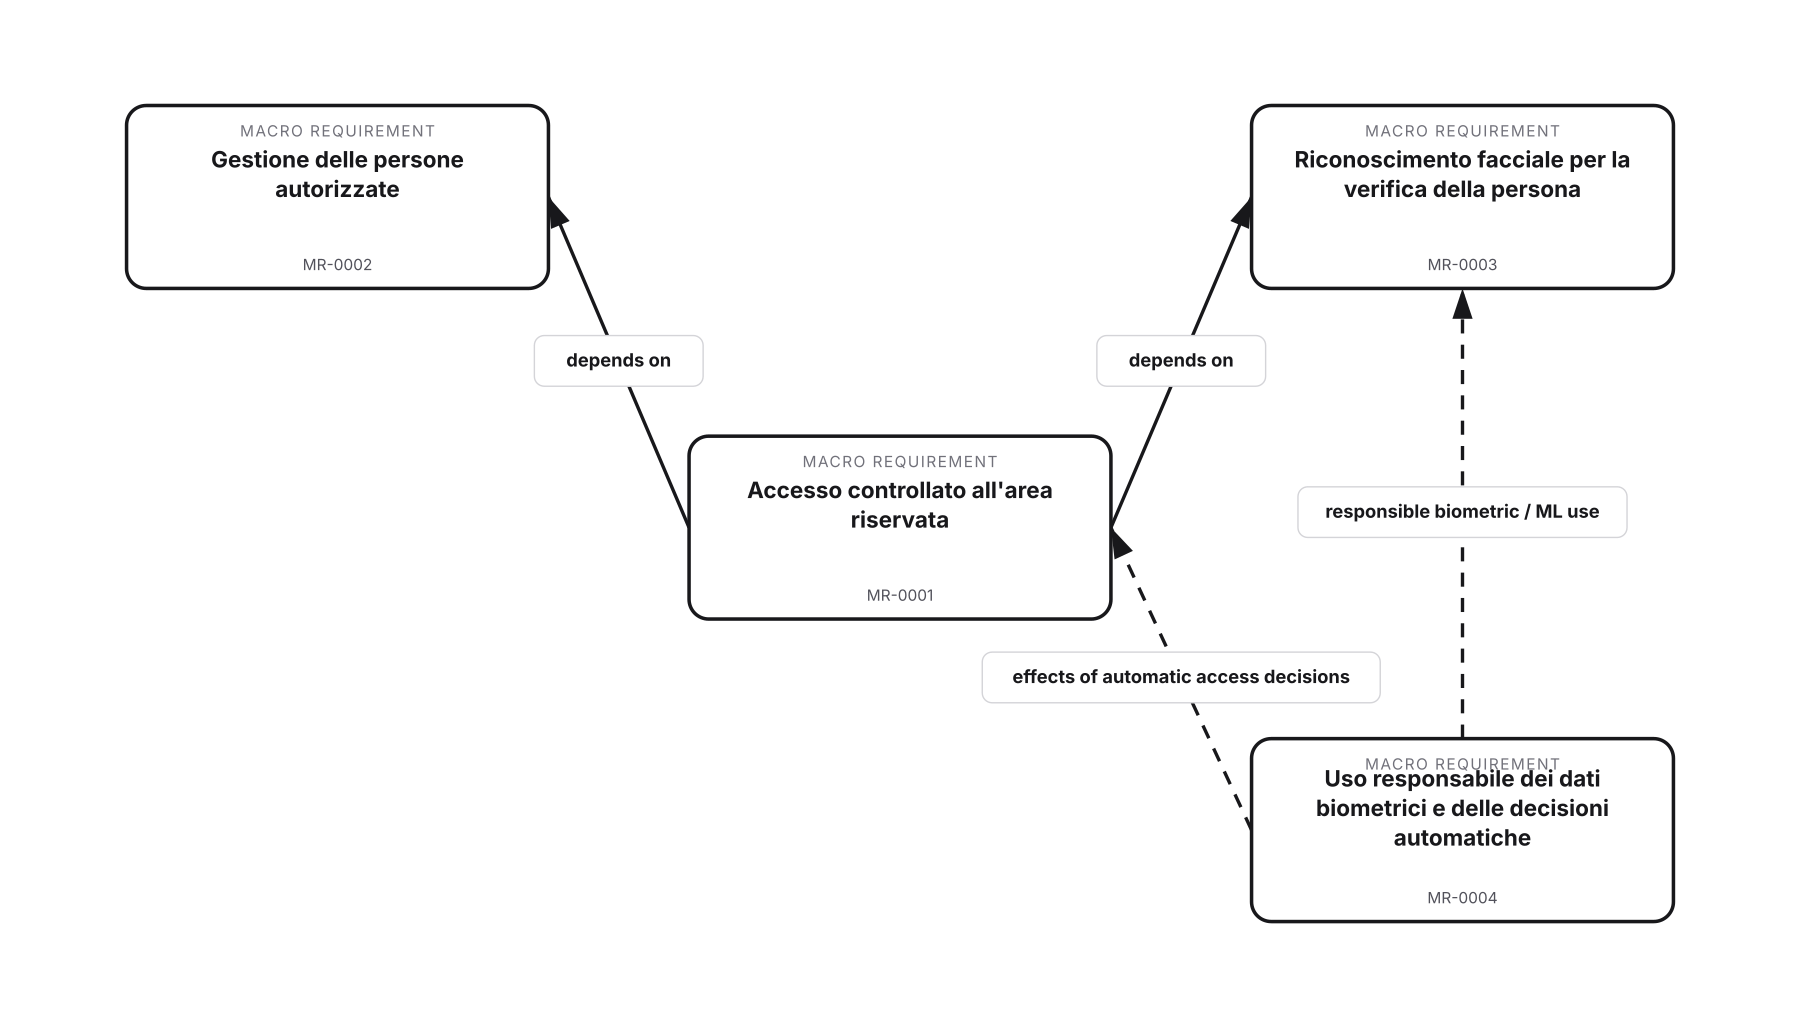
\includegraphics{facial-access-macro-project-map.png}

The two solid links are explicit \texttt{dependsOn} relations from the
access-control concern. The dashed links show a reviewed teaching
interpretation of how the responsible-biometric/automatic-decision
concern cuts across recognition and access effects. These dashed links
are deliberately \textbf{not canonical MR topology}.

Textual reading:

\begin{enumerate}
\def\labelenumi{\arabic{enumi}.}
\tightlist
\item
  controlled access depends on knowing who is authorized;
\item
  controlled access also depends on verifying the person;
\item
  biometric recognition and its automatic consequences raise a distinct
  responsible-use concern;
\item
  none of these statements determines where inference runs, which
  protocol is used or how devices are connected.
\end{enumerate}

\subsection{ThreatForge example}\label{threatforge-example}

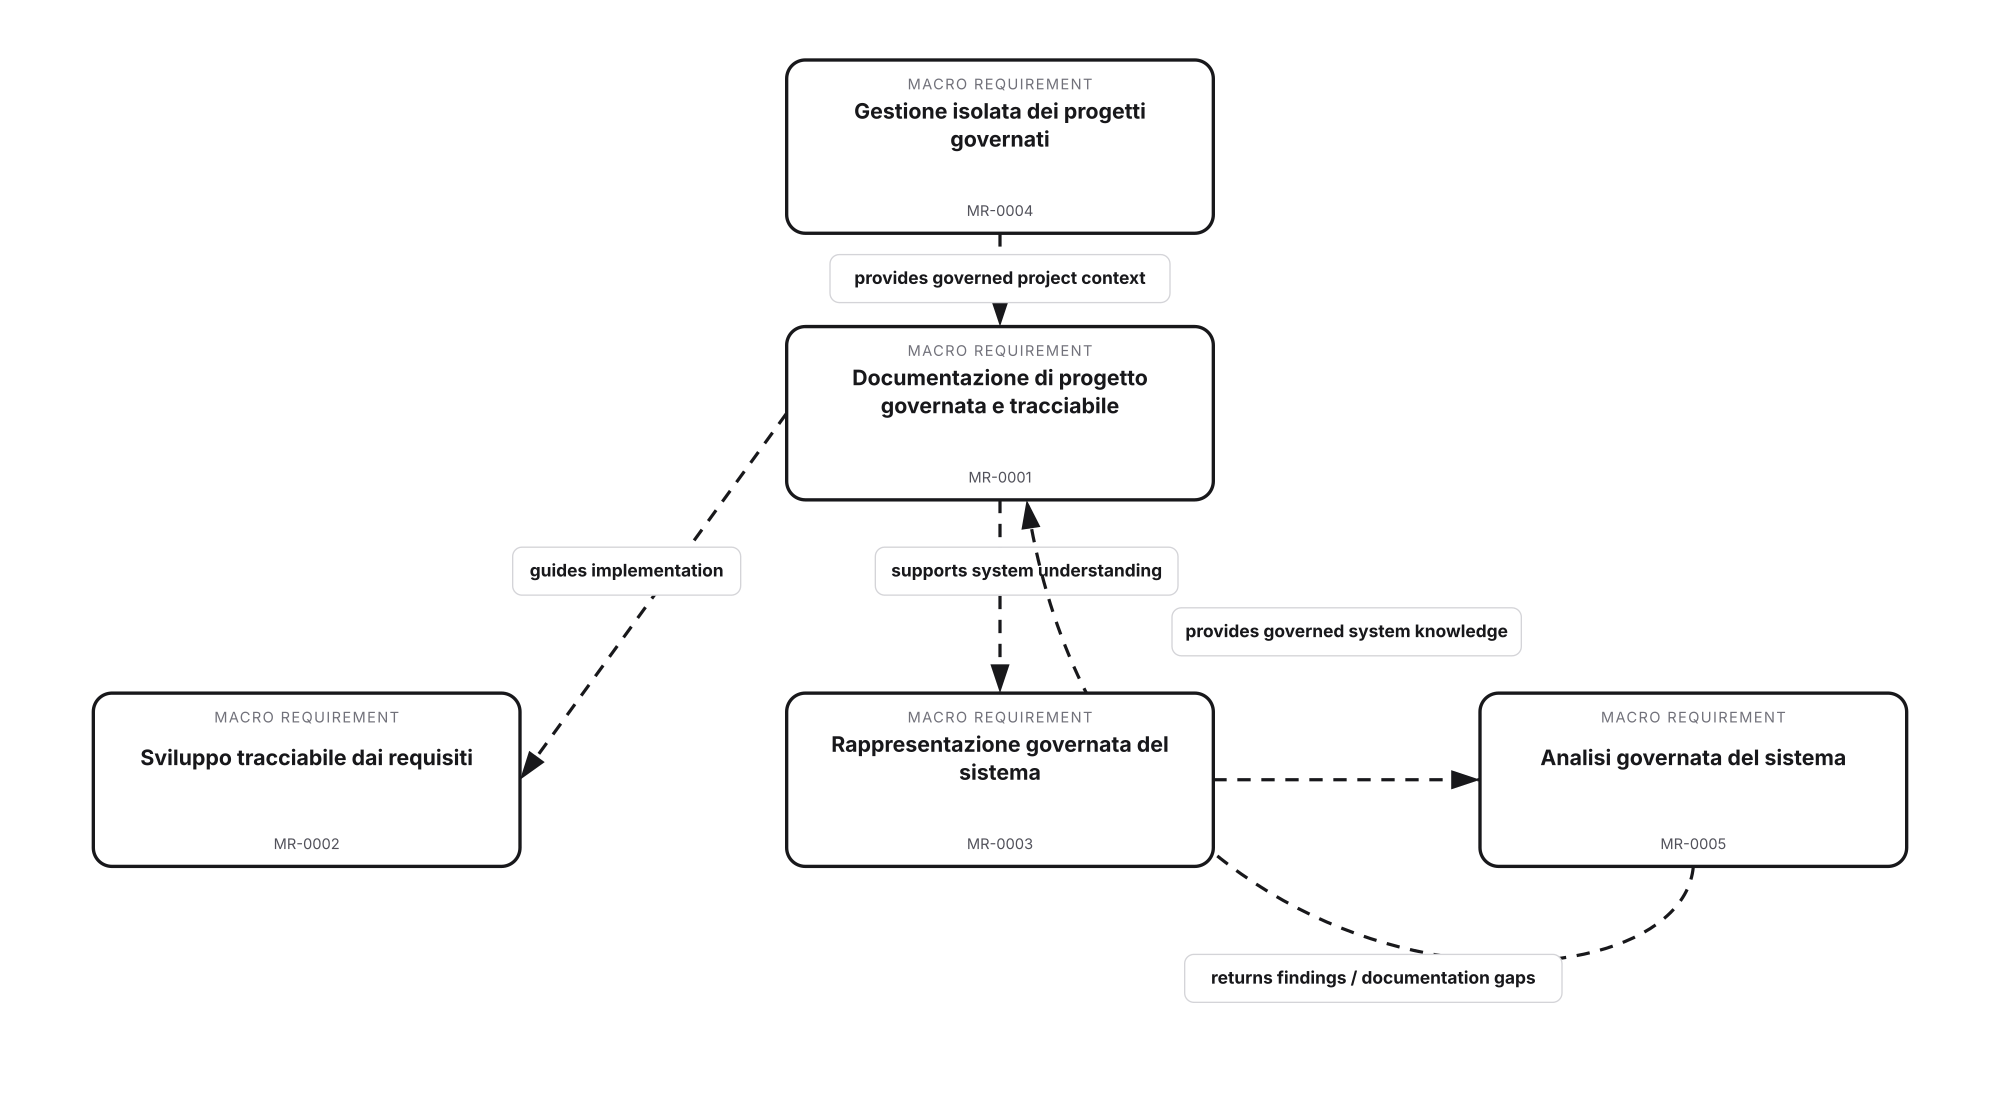
\includegraphics{threatforge-macro-project-map.png}

ThreatForge\textquotesingle s current candidate MR set can be taught as
a macro cycle:

\begin{enumerate}
\def\labelenumi{\arabic{enumi}.}
\tightlist
\item
  ThreatForge governs isolated projects;
\item
  governed documentation carries project knowledge;
\item
  that knowledge guides implementation and supports a governed
  representation of the system;
\item
  the representation can be analyzed through different methods;
\item
  analysis findings/documentation gaps return to the governed
  documentation lifecycle.
\end{enumerate}

The candidate MR corpus does not currently encode all these explanatory
links as explicit \texttt{dependsOn} records, so the ThreatForge map
marks them as \textbf{non-canonical didactic interpretations}. This is
useful evidence for the teachability test, not permission to silently
create canonical relations.

\subsection{Teachability test}\label{teachability-test}

An MR set passes the working teachability test when a domain-competent
reader new to the project can use the MRs to answer, without lower-level
architecture:

\begin{itemize}
\tightlist
\item
  What are the project\textquotesingle s main concerns?
\item
  Why does each concern exist?
\item
  How do the macro concerns collaborate or depend on each other?
\item
  Can the reader explain the project\textquotesingle s macro functioning
  from the map and textual equivalent?
\item
  Would the explanation remain valid after a lower-level design Decision
  changes?
\end{itemize}

\subsection{Accessibility / BES-oriented
presentation}\label{accessibility--bes-oriented-presentation}

The maps deliberately use:

\begin{itemize}
\tightlist
\item
  few blocks;
\item
  canonical titles;
\item
  one idea per block;
\item
  labeled edges;
\item
  no color-only semantics;
\item
  textual equivalent and traceability in the HTML companions;
\item
  progressive disclosure from MR map to later
  Decision/Requirement/system/analysis views.
\end{itemize}

\subsection{Rendering consistency with ThreatForge
DFDs}\label{rendering-consistency-with-threatforge-dfds}

The ThreatForge DFD renderer at planning SHA
\texttt{44f77796469465a6a076596b1b1ba1afdde92db7} is a custom
deterministic HTML/SVG renderer with renderer-neutral semantic input.
The MR study maps imitate that visual/accessibility language but keep
their own semantics. See
\texttt{MR\_MAP\_RENDERING\_COMPATIBILITY\_NOTE.md}.

\subsection{Files in this folder}\label{files-in-this-folder}

\begin{itemize}
\tightlist
\item
  \texttt{facial-access-macro-project-map.projection.json} -
  renderer-neutral study projection;
\item
  \texttt{facial-access-macro-project-map.html} - accessible
  self-contained teaching view;
\item
  \texttt{facial-access-macro-project-map.svg} / \texttt{.png} - static
  visual companions;
\item
  \texttt{threatforge-macro-project-map.projection.json} -
  renderer-neutral study projection;
\item
  \texttt{threatforge-macro-project-map.html} - accessible
  self-contained teaching view;
\item
  \texttt{threatforge-macro-project-map.svg} / \texttt{.png} - static
  visual companions;
\item
  \texttt{MR\_MAP\_RENDERING\_COMPATIBILITY\_NOTE.md} - inspected
  ThreatForge DFD rendering pattern and future reuse direction.
\end{itemize}

\end{document}
